\chapter{Results}
In this chapter our results are presented. Starting off with a description f the graph database, we then move on to the three different cases. 

\section{Graph Database}
% Power of graph databases
We are dealing with connected data, where choosing a graph database have two advantages according to \citet{robinson2013}: performance and flexibility. In a relational database, the join-intensive query performance deteriorates as the dataset gets larger while, with a graph database the performance remains relatively constant. This is due to the fact that a query is only localized to a fraction of the graph making the run time proportional to the size of the sub-graph related to the query rather than the overall graph containing all available data.

Furthermore, there is the aspect of flexibility. Graphs are naturally additive \cite{robinson2013} such that new sub-graphs can be added containing more nodes and edges and new relations can be introduced as the understanding of the dataset grows. This have a positive implication for the analysts that does not have to model the domain in exhaustive detail from the start but can add information as time progress. 

Thus, according to the motivation above, we have created a graph database in Neo4j, a cloud based graph database supporting some basic analysis through their query language Cypher.

\section{Gh0st RAT Controllers}
In this section, we present the AUC values and the maximal measured F$_1$ score for the different indices and different numbers of reference nodes that the similarity is based on. We first present the results for the first dataset and then move on the the second dataset. Since cross validation is performed, 20 trials has been carried out. However, we first motivate out choice of parameters for the Local Path index and Katz index.

\textbf{Choice of parameters.} For the Local Path index and Katz index,  the parameter $\alpha$ had to be chosen. To do so, different values of alpha  tried and evaluated based on the resulting AUC and F$_1$ values. For the Local Path index, found that the performance was lowered with an increasing value of $\alpha$. Thus, to make the most fair comparison as possible, a low value of alpha was chosen, namely 0.01. For the global index, the Katz index, a maximization of performance was found for $\alpha=0.5$. These values of the discounting factor $\alpha$ was used throughout the simulations. 

\textbf{The first dataset.} The result for the first dataset in the RAT controller case is given in table \ref{aucIndex}. We find small variance in the results for the local indices. The quasi-local Local Path index and the global Katz index perform worse than the local ones. The best overall performance if found when using 4-5 reference nodes. The best F$_1$ value is then given by 98 \% and an AUC of approximately 96 \%. 

\begin{table}[h!]
    \centering
    \caption{AUC and F$_1$ score for different number of reference nodes. The AUC is calculated from the precision-recall curve. The F$_1$ score represents the average accuracy between the 20 runs.}
    \begin{tabular}{|c||c|c||c|c||c|c||c|c||c|c|}
      \hline
      \multirow{2}{*}{~} 
            & \multicolumn{2}{c||}{1}
            & \multicolumn{2}{c||}{2}
            & \multicolumn{2}{c||}{3}
            & \multicolumn{2}{c||}{4}
            & \multicolumn{2}{|c|}{5} \\             \cline{2-11}
      ~     &AUC&F$_1$&AUC&F$_1$&AUC&F$_1$&AUC&F$_1$&AUC&F$_1$ \\ \hline
    Dice    &0.8995 & 0.89 & 0.9363 &0.94 &0.9554&0.97 & 0.9627 &0.98&0.9658 & 0.98 \\
    Jaccard &0.8978 & 0.89 & 0.9367 &0.94 &0.9552&0.97 & 0.9616 &0.98&0.9654 & 0.98 \\
    Cosine  &0.8943 & 0.89 & 0.9337 &0.94 &0.9518&0.97 & 0.9591 &0.98&0.9621 & 0.98 \\
    ProHub  &0.8850 & 0.89 & 0.9244 &0.94 &0.9435&0.97 & 0.9478 &0.98&0.9434 & 0.98 \\
    DeHub   &0.8987 & 0.89 & 0.9378 &0.94 &0.9563&0.97 & 0.9631 &0.98&0.9664 & 0.98 \\
    LP      &0.6169 & 0.52 & 0.8365 & 0.85 & 0.8505 & 0.88 & 0.9024 & 0.92 & 0.9009 & 0.91 \\ 
    Katz    &0.2233 & 0.11 & 0.2336 & 0.11 & 0.1958 & 0.11 & 0.1781 & 0.11 & 0.1566 & 0.20 \\ \hline
    \end{tabular}
    \label{aucIndex}
\end{table}

Futhermore, there were three IP addresses that were constantly classified as RAT controllers, while they in fact were annotated as \textit{Non-ghost}s. Performing 100 trials for each case of using 1-5 reference nodes, the IP addresses were classified as RAT controllers in the majority or all of the times. Using only one reference node, the three different IP addresses were classified as RAT controller in 76 \%, 97 \% and 95 \% of the times, respectively. Using two reference nodes, they were classified as RAT controller in 95 \%, 99 \% and 99 \% of the times. Using 3-5 reference nodes, all three IP addresses were classified as RAT controllers in every one of the 100 trials. Because of this, there exists reason to believe they are falsly annotated. 

\textbf{The second dataset.} The second data set was much more sparse of RAT controllers. Of 10091 nodes, only 32 were identified as RAT controllers. Performing the exact same analysis on this data set as the previous one gave us the result shown in table \ref{aucIndex2}.

\begin{table}[h!]
    \centering
    \caption{AUC and F$_1$ score for different number of reference nodes. The AUC is calculated from the precision-recall curve. The F$_1$ score represents the average accuracy between the 20 runs.}
    \begin{tabular}{|c||c|c||c|c||c|c||c|c||c|c|}
      \hline
      \multirow{2}{*}{~} 
            & \multicolumn{2}{c||}{1}
            & \multicolumn{2}{c||}{2}
            & \multicolumn{2}{c||}{3}
            & \multicolumn{2}{c||}{4}
            & \multicolumn{2}{|c|}{5} \\             \cline{2-11}
      ~     &AUC&F$_1$&AUC&F$_1$&AUC&F$_1$&AUC&F$_1$&AUC&F$_1$ \\ \hline
    Dice    & 0.9696 & 0.98 & 0.9680 & 1.00 & 0.9531 & 1.00 & 0.9375 & 1.00 & 0.9219 & 1.00 \\
    Jaccard & 0.9696 & 0.98 & 0.9680 & 1.00 & 0.9531 & 1.00 & 0.9375 & 1.00 & 0.9219 & 1.00 \\
    Cosine  & 0.9696 & 0.98 & 0.9680 & 1.00 & 0.9531 & 1.00 & 0.9375 & 1.00 & 0.9219 & 1.00 \\
    ProHub  & 0.9696 & 0.98 & 0.9680 & 1.00 & 0.9531 & 1.00 & 0.9375 & 1.00 & 0.9297 & 1.00 \\
    DeHub   & 0.9696 & 0.98 & 0.9680 & 1.00 & 0.9531 & 1.00 & 0.9375 & 1.00 & 0.9219 & 1.00 \\ 
    LP      & 0.7930 & 0.78 & 0.9283 & 0.96 & 0.9279 & 0.96 & 0.9426 & 0.98 & 0.9206 & 0.98 \\ 
    Katz    & 0.1888 & 0.29 & 0.1960 & 0.28 & 0.1949 & 0.26 & 0.1759 & 0.28 & 0.1850 & 0.27 \\ \hline
    \end{tabular}
    \label{aucIndex2}
\end{table}

In the second dataset, no falsely annotated IP addresses were found. 

\nopagebreak
\FloatBarrier
\section{Classification of malicious IP addresses}
Below, the results of the feature classifier is presented. 

\textbf{All six features.} Including all the six features in the model, the best accuracy was found for the parameters $C=10$ and $\gamma=50$. The results for the SVM, using six features, are presented in table \ref{IpRes}. The table presents results, based on 20 repetitions, with a confidential level of 95 \%. The SVM classifier, based on all 6 input features, performed prediction with an accuracy of about 75.1 \%. Futhermore, 7.4 \% of the predicted classes were higher than Recorded Future's while 17.5 \% were lower. 

\begin{table}[h!]
    \centering
    \caption{Results from the SVM classifier using six features. The table shows the fraction of correct predictions (accuracy), the fraction of higher predictions and the fraction of lower predictions in relation to Recorded Future's actual classification.}
    \begin{tabular}{|c|c|}
    \hline
        \multicolumn{2}{|c|}{SVM with 6 features}\\ \hline
        Correct classification  & 0.7510 $\pm$0.0238 \\
        Higher classification   & 0.0736 $\pm$0.0293 \\
        Lower classification    & 0.1753 $\pm$0.0450 \\ \hline
    \end{tabular}
    \label{IpRes}
\end{table}



\textbf{Two features.} Using only two features in the model, the best accuracy was found for $C=10$ and $\gamma=10$. However, it should be pointed out that the distribution of predicted classes only included 4 of the 5 classes. The results from including only the two topological features are presented in table \ref{IpRes2Feat}. The features were PageRank and degree of the node. The table presents results, based on 20 repetitions, with a confidential level of 95 \%. The SVM classifier, based on 2 input features, performed prediction with an accuracy of about 60.7 \%. Futhermore, 0.3 \% of the predicted classes were higher than Recorded Future's while 38.9 \% were lower. 

\begin{table}[h!]
    \centering
    \caption{Results from the SVM classifier using two features. The table shows the fraction of correct predictions (accuracy), the fraction of higher predictions and the fraction of lower predictions in relation to Recorded Future's actual classification.}
    \begin{tabular}{|c|c|}
    \hline
        \multicolumn{2}{|c|}{SVM with 2 features}\\ \hline
        Correct classification  & 0.6072 $\pm$ 0.0083 \\
        Higher classification   & 0.0034 $\pm$ 0.0032 \\
        Lower classification    & 0.3894 $\pm$ 0.0092 \\ \hline
    \end{tabular}
    \label{IpRes2Feat}
\end{table}

\textbf{Four features.} Using four features in the model, the best accuracy was found for $C=100$ and $\gamma=100$. All classes of maliciousness were represented in the predictions. The results from including only four features are presented in table \ref{IpRes4Feat}. The features included information about the number of hits and the neighbours co-occurrence with malwares, cyber vulnerabilities and attack vectors. The features were PageRank and degree of the node. The table presents results, based on 20 repetitions, with a confidential level of 95 \%. The SVM classifier, based on 4 input features, performed prediction with an accuracy of about 74.0 \%. Futhermore, 8.3 \% of the predicted classes were higher than Recorded Future's while 17.7 \% were lower. 

\begin{table}[h!]
    \centering
    \caption{Results from the SVM classifier using four features. The table shows the fraction of correct predictions (accuracy), the fraction of higher predictions and the fraction of lower predictions in relation to Recorded Future's actual classification.}
    \begin{tabular}{|c|c|}
    \hline
        \multicolumn{2}{|c|}{SVM with 4 features}\\ \hline
        Correct classification  & 0.7397 $\pm$ 0.0170 \\
        Higher classification   & 0.0829 $\pm$ 0.0531 \\
        Lower classification    & 0.1774 $\pm$ 0.0477 \\ \hline
    \end{tabular}
    \label{IpRes4Feat}
\end{table}

\textbf{Random classifier.} For a pseudorandom classifier, the results can be found in table \ref{randClass}. We have found an accuracy of 20 \%, which was to be expected. However, 70 \% of the predictions gave a higher risk classification and 10 \% gave a lower risk classification.

\begin{table}[h!]
    \centering
    \caption{Results from the a random classifier, based on a uniform distribution. The table shows the fraction of correct predictions (accuracy), the fraction of higher predictions and the fraction of lower predictions in relation to Recorded Future's actual classification.}
    \begin{tabular}{|c|c|}
    \hline
        \multicolumn{2}{|c|}{Random classifier}\\ \hline
        Correct classification & 0.2002 $\pm$ 0.0022 \\
        Higher classification  & 0.6994 $\pm$ 0.0023\\
        Lower classification   & 0.1003 $\pm$ 0.0017\\ \hline
    \end{tabular}
    \label{randClass}
\end{table}

\FloatBarrier
\section{Prediction of Future Cyber Attacks}
The AUC and prediction rate of predicting future cyber attacks using PLP on the data set described in \secref{cyberattacks} is shown in \figref{fig:plp_auc} for different lengths of the set used for testing.
\begin{figure}[!ht]
\centering
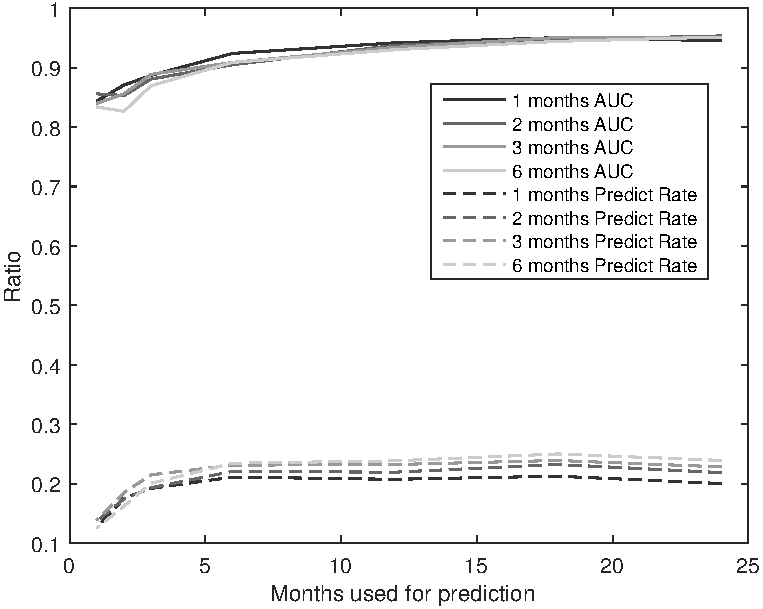
\includegraphics[scale=0.9]{images/auc_plp_result.pdf}
\caption{\label{fig:plp_auc} AUC and Prediction rate for the PLP algorithm used on the cyber attack bipartite graph. The different shades of grays represent differents length of time period used for testing (in months). AUC was calculated according to the description in section \ref{plp:auc} and prediction rate according to \ref{plp:predict_rate}.}
\end{figure}

How great the natural limitations of the algorithm are can be seen in \figref{fig:plp_max} where the maximum possible prediction rate, the ratio of cyber attacks with same actors as was previously seen in the prediction set and the ratio of cyber attacks that involved at least one new actor is presented.

\begin{figure}[!ht]
\centering
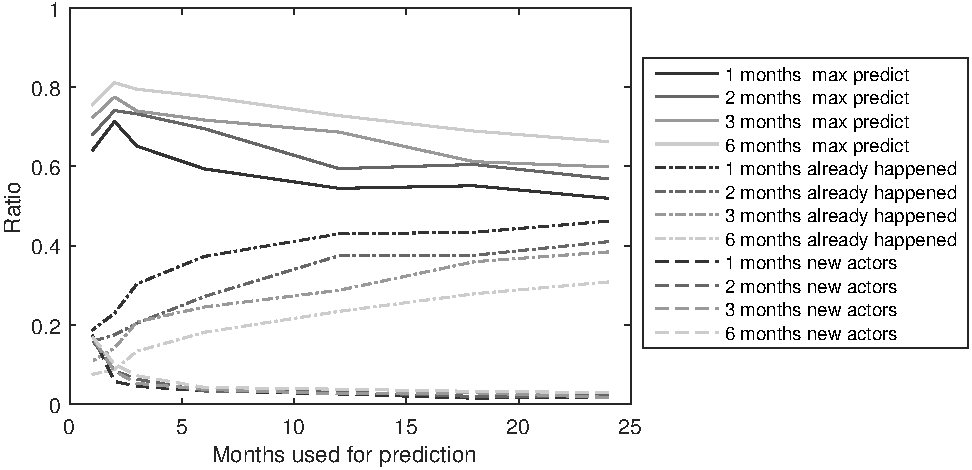
\includegraphics[width=\textwidth]{images/max_plp_result.pdf}
\caption{\label{fig:plp_max} 
Maximum prediction rate possbile for PLP for comarison with the prediction rate in \figref{fig:plp_auc}. Also showing the ratio of attacks with set of actors already in prediction set as well as the ratio of attacks involving at least one new actor.}
\end{figure}

We find that the auc increases around 10 percent units from 1 month of prediction data to 24 months of prediction data. However, the prediction rate does not vary that much for length of prediction data of at least 6 months.

